\part{Conception}

%%%%%%%%%%%%%%%%%%%%%%%%%%%%%%%%%%%%%%%%%%%%%%%%%%%%%%%%%%%%
\section{Rappel du contexte}
La suite de ce document présente la démarche de conception entreprise dans le
cadre de ce projet. Nous souhaitons proposer un éditeur de textes page capable
de manipuler efficacement un fichier texte séquentiel de longueur variable.

L'architecture retenue à l'issue de cette phase de conception doit permettre
d'offrir un outil ergonomique (aspect essentiellement traité dans le cadre de
la spécification), portable sur différents environements et différentes architectures, maintenable et
efficace. Nous devons garder en mémoire que cet outil doit pouvoir être déployé
dans un environnement où les ressources sont limitées.

Nous analyserons et critiquerons trois solutions de gestion des données en
mémoire centrale et mémoire secondaire selon les critères de portabilité,
maintenabilité et efficacité. Nous retiendrons celle jugée la plus pertinente
et nous la décrirons en détail.



%%%%%%%%%%%%%%%%%%%%%%%%%%%%%%%%%%%%%%%%%%%%%%%%%%%%%%%%%%%%
\section{Choix d'une solution}
\subsection{Présentation des alternatives}

\subsubsection{Points commun des trois solutions}
% Yoann
À l'ouverture d'un fichier, son contenu est copié dans un fichier temporaire --- éventuellement en le structurant de manière adaptée à l'éditeur. Le fichier est indexé de manière à pouvoir accéder aux lignes directement.

Un tampon de taille limitée est créé en mémoire centrale. Lorsque l'utilisateur demande à accéder à des lignes qui n'y sont pas encore chargées, les lignes les plus anciennement accédées sont remplacées par celles qui viennent d'être demandées.

Le tampon est modifié directement au fur et à mesure de la frappe de l'utilisateur, et la ligne modifiée est transférée dans le fichier temporaire dès que l'utilisateur passe à une nouvelle ligne ou demande une sauvegarde du fichier. Le fichier source, quant à lui, est mis à jour sur demande de l'utilisateur (sauvegarde du fichier).

\subsubsection{Solution 1 : structure consécutive}
% Paul
Toute la mémoire est allouée dans des tableaux, d'un seul bloc.

Le fichier temporaire est lui aussi placé dans une structure consécutive dans
un zone contigüe de la mémoire centrale.

La solution est donc homogène : le même mécanisme est mis en place entre la
mémoire centrale et la mémoire secondaire. La compréhension du système est
alors simplifiée.

L'accès est direct : chaque caractère du texte peut être accédé en tant
constant ($O(n)$). De fait, si l'on a besoin uniquement de remplacer des
caractères par d'autres caractères, cette solution est efficace.

De la même manière, si l'on a besoin de rajouter des caractères à la fin du
texte, la solution est là encore très efficace, dans les limites de la mémoire
disponible sur le système.

De plus, cette solution présente l'avantage de ne pas devoir réserver de la
mémoire pour le chaînage, celui-ci n'étant pas présent dans cette solution.
Par contre, nous devons impérativement réserver un \emph{buffer} de taille
importante dès le début, pour éviter la réallocation intempestive. Nous
pourrions envisager d'utiliser la technique bien connue de la réallocation par
pas de $n^2$, c'est à dire réserver la mémoire selon un schéma quadratique, et
donc réserver de plus en plus de mémoire à chaque réallocation.

Par contre, si l'on a besoin d'insérer des caractères au milieu du texte, la
solution est très couteuse. En effet chaque insertion ou suppression de
caractères provoque des opérations en $O(n)$ (où $n$ est le nombre de
caractères entre le point de fin d'insertion ou de suppression et la fin de la
mémoire allouée (le \emph{buffer}). Comme il s'agit d'une opération assez
classique et fréquente, de nombreuses opération sont à prévoir.  Ces opération
sont du type \texttt{memmove()}, qui permet de déplacer des données dans un
\emph{buffer}, et qui a une complexité de $n$.

\subsubsection{Solution 2 : structure mixte}
% Martin
La seconde solution proposée est une variation de la première. La structure de
données en mémoire secondaire reste identique : nous conservons le fichier sous
la forme d'une structure de caractères contigüs. Cependant, le bloc texte est
fragmenté en sous-blocs de taille donnée en mémoire centrale et stockée dans
des éléments d'une liste doublement chaînée. Les éléments sont chaînés dans
l'ordre des données du fichier.

La structure d'un élément de la liste contiendra les données suivantes :
\begin{description}
  \item[@précédant] Adresse de l'élément précédant dans la liste,
  \item[@suivant] Adresse de l'élément suivant dans la liste,
  \item[lgUtil] Longueur du bloc utilisée données,
  \item[lgMax] Longueur totale du bloc de données,
  \item[info] Bloc de données (contient le fragment de texte stocké dans
l'élément).
\end{description}

Le bloc de données peut éventuellement être plus large que la chaîne de
caractères qu'il contient. En effet, lors de l'édition du document, de nouveaux
blocs peuvent être alloués mais pas intégralement remplis par la saisie de
l'utilisateur. Il est donc nécessaire de retenir deux informations sur ce bloc
: $lgUtil$, la longueur effectivement utilisée, qui correspond à la taille de
la chaine stockée (marqueur de chaîne inclu),  et $lgMax$, la taille du bloc
$info$.

Cette seconde solution est moins efficace que la première lors du chargement et
de la sauvegarde du fichier. Les structures manipulées en mémoire centrale et
mémoire secondaire ne seront plus homogènes, il sera donc nécessaire de
proposer des procédures permettant de convertir le bloc de texte d'un format de
structure à l'autre. Les opérations de chargement et sauvegarde du fichier
seront plus coûteuses du fait de ces opérations de traduction, mais aussi des
opérations d'allocation de mémoire proportionnelles à la taille du fichier.

Par ailleurs, cette solution est plus coûteuse en espace pour la mémoire
centrale, puisqu'il est nécessaire de prévoir quelques octets correspondant à
la taille des pointeurs manipulés.

En contrepartie, cette solution offre de biens meilleurs temps d'accès en
lecture et écriture, puisqu'il est possible de naviguer d'un élément de la
chaîne à un autre sans lire l'ensemble du bloc. La complexité algorithmique
d'une telle opération sera en $O(n/m)$, où n est la longueur maximale d'un bloc
et m le nombre d'éléments de la chaîne. L'insertion de texte nécessite de se
placer à la fin du bloc de données et d'ajouter le caractère saisi. Si la
longueur de la chaîne atteint la longueur maximale, il sera nécessaire
d'allouer un nouvel élément et de l'insérer dans la chaîne à la suite de
l'élément courant.

Une double liste chaînée est une structure de données classique qui n'est pas
difficile à implémenter et à manipuler. L'impact d'une telle solution sur la
maintenabilité est très faible.

\subsubsection{Solution 3 : structure chaînée}
% Yoann
Toutes les structures de données sont chaînées.

Le ficher temporaire est chaîné grâce à des adresses virtuelles, comme présentées ci-dessous.

\begin{figure}[H]
	\centering
	\caption{Structure d'une adresse virtuelle}
	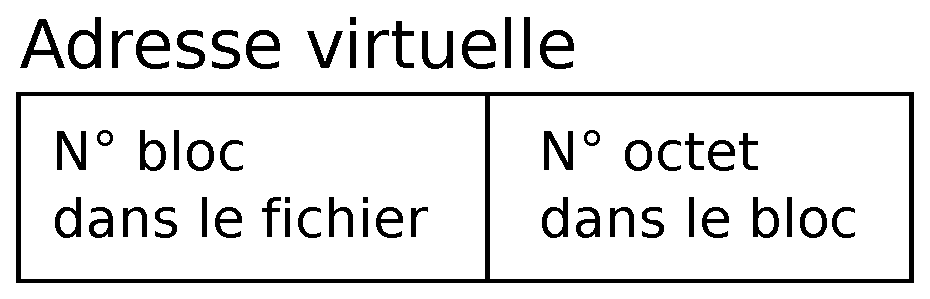
\includegraphics[width=0.5\textwidth]{structure_chainee_temp_adresse_virtuelle}
\end{figure}

Ainsi chaque ligne (y compris la \og ligne 0 \fg virtuelle) fait référence à son successeur et son prédécesseur. On stocke également la longueur de l'information (\og longueur utile \fg) et le nombre d'octets disponibles dans l'enregistrement (\og longueur max \fg, supérieure ou égale à la longueur utile).

\begin{figure}[H]
	\centering
	\caption{Structure du fichier temporaire de la solution 3}
	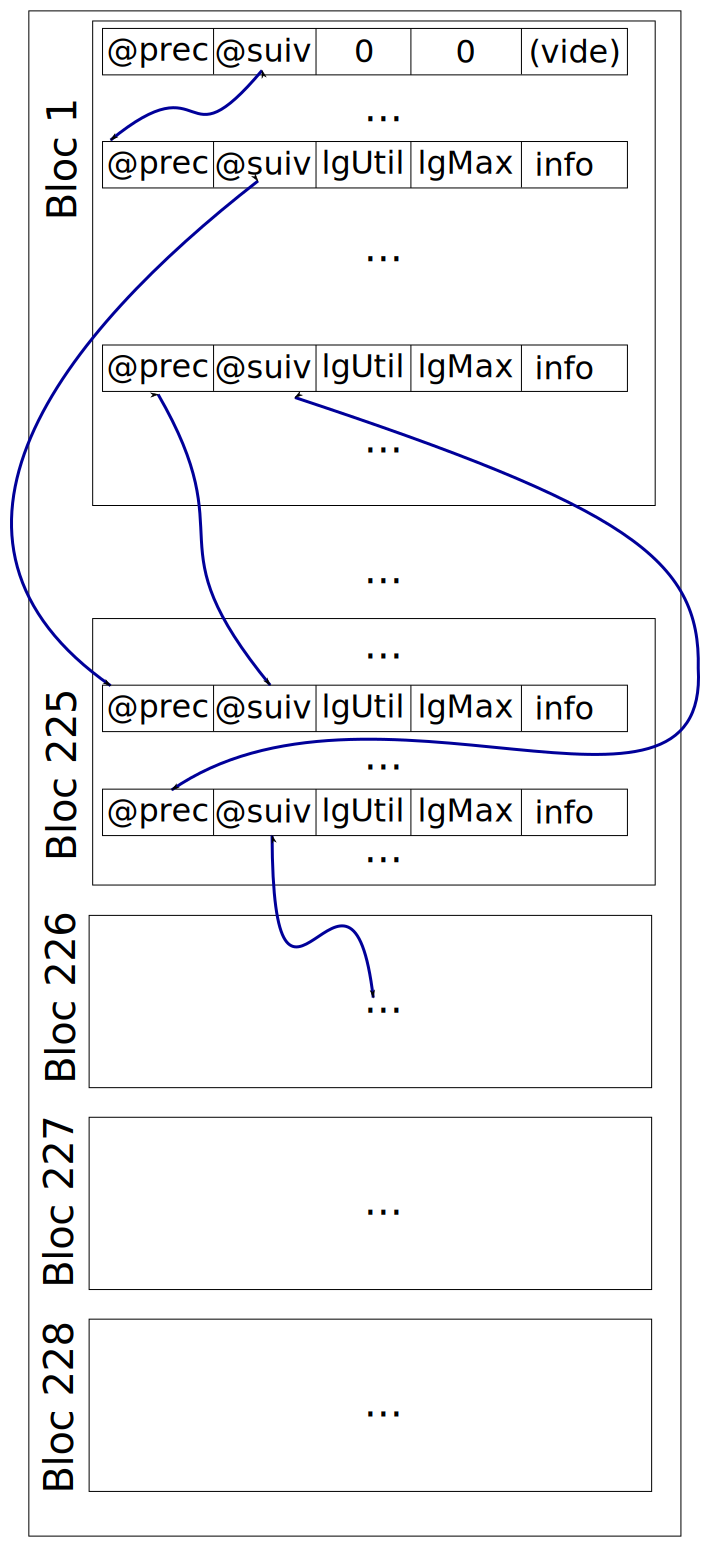
\includegraphics[width=0.6\textwidth]{structure_chainee_temp}
\end{figure}

L'accès direct (lorsque l'utilisateur demande d'accéder à la ligne $l$, par exemple) est possible toutes les $L$ lignes ($L$ à définir) grâce à la table de \textsl{mapping}, qui donne pour chaque bloc la dernière ligne stockée dans celui-ci. Cette table est bien sûr complétée et mise à jour au fur et à mesure de l'édition du fichier (suppressions, ajouts, \ldots). Pour accéder à une ligne non indexée, il suffit d'accéder à une ligne proche et indexée, et de suivre le chaînage (complexité bornée).

Cette table contient bien sûr d'autres informations, comme le montre la représentation suivante.

\newcommand{\TableSolTroisHLine}{\cline{1-5} \cdashline{6-6} \cline{7-7}}
\begin{figure}[H]
	\centering
	\caption{Structure de la table de \textsl{mapping} de la solution 3}
	\vspace{3mm}
	\begin{tabular}{|c|c|c|c|c|c|c|}
		N\textdegree{} ligne & N\textdegree{} bloc & Octet & Chargé & Date dernier accès & (Autres infos) & Adresse MC \\
		\TableSolTroisHLine
		10 & 1 & 156 & Non & 1289135888657534079 & \ldots & \texttt{0x000000}\\
		\TableSolTroisHLine
		\multicolumn{7}{:c:}{} \\
		\multicolumn{7}{:c:}{\ldots} \\
		\multicolumn{7}{:c:}{} \\
		\TableSolTroisHLine
		119 & N & 451 & Oui & 1289135888658945079 & \ldots & \texttt{0x4006d4}\\
		\TableSolTroisHLine
	\end{tabular}
\end{figure}




\subsection{Comparaison des alternatives}
% En commun
% « Mécanisme de justification » : un tableau avec des « + » et des « - » ?

Les critères d'ergonomie et de portabilité ne sont pas pertinents pour la
comparaison des alternatives.
En effet, une bonne ergonomie, au niveau de la conception, sera traduite par une
bonne efficacité, afin d'éviter à l'utilisateur des attentes inutiles.
De plus, nous n'utiliserons pas d'assembleur dans les différentes solutions, se
reposant sur le compilateur C++ pour assurer cette portabilité. Le système sera
donc portable tant que la plateforme dispose d'un compilateur C++.

Nous avons choisis de pondérer ces critères, pour prendre en compte leur
importance respectives.

\begin{table}[H]
	\centering
	\begin{tabular}{l c|c|c|c}
		Critère & Pondération & Solution 1 & Solution 2 & Solution 3 \\
		\hline \hline
		Maintenabilité & 20 & ++ (34) & ++ (35) & +++ (56) \\
		\hline
		Décomposable en couches & 8 & + & ++ & +++ \\
		Homogénéité & 5 & +++ & + & +++ \\
		Couplage entre couches & 5 & + & ++ & +++ \\
		Facilité d'implémentation & 2 & +++ & ++ & + \\
		\hline \hline
		Efficacité & 15 & ++ (27) & ++ (27) & +++ (41) \\
		\hline
		Complexité en insertion & 3 & + & ++ & +++ \\
		Complexité en suppression & 3 & + & ++ & +++ \\
		Complexité au changement de ligne & 3 & + & + & +++ \\
		Complexité de changement de page & 3 & +++ & ++ & +++ \\
		Économie mémoire & 1 & +++ & ++ & + \\
		Complexité de chargement du fichier temporaire & 1 & +++ & ++ & +++ \\
		Complexité de la sauvegarde & 1 & +++ & ++ & + \\
		\hline
		Total & 35 & 61 & 60 & 98 \\
	\end{tabular}
	\vspace{0.5cm}
	\caption{Table comparative des avantages et inconvénients de chaque solution}
\end{table}



%%%%%%%%%%%%%%%%%%%%%%%%%%%%%%%%%%%%%%%%%%%%%%%%%%%%%%%%%%%%
\section{Détail de la solution choisie}

\subsection{Mécanisme de stockage en mémoire secondaire permettant l'accès direct}
% Yoann

\subsection{Structuration d'une ligne en mémoire secondaire et en mémoire
    centrale}
% Yoann

\subsection{Gestion des blocs sur la mémoire secondaire pour faire de l'accès
    direct}
% Martin

\subsection{Gestion de l'espace libre}
% Paul

\section{Proposition d'architecture}
% Paul
% Découpage modulaire et hiérarchique


%%%%%%%%%%%%%%%%%%%%%%%%%%%%%%%%%%%%%%%%%%%%%%%%%%%%%%%%%%%%
\section{Bilan}
% Martin
% Bilan de la solution choisie par rapport aux exigeances + réflexions personnelles
